\section{Introduction}
In molecular dynamics, a thermostat is an algorithm built with the purpose of generating samples from a statistical ensemble at constant temperature $T$.
At this point, we know that the typical choice among the statistical ensembles, when simulating a real physical system, is the Canonical one, which allows fluctuations of the total energy under the constraint that its average remains constant over time.
Therefore, our aim will be to build thermostats which sample configurations drawn from the Canonical ensemble. 

Before entering in the implementation of these algorithms, let's recall some of the main features of the ensemble we are interested in.

\subsection{Recap of the Canonical ensemble}
The probability distribution related to the Canonical ensemble, as defined in Chapter 1 (1.36), is given by
\begin{equation}
     P(x)=\frac{e^{-\beta H(x)}}{Z}
\end{equation}
with 
\begin{equation}
     Z=\int_ {}^{} e^{-\beta H(x)}dx
\label{zetafunc}
\end{equation} 

\par Is important to remember that here $x$ represents a vector that contains the position and momenta of all the particles of the system, so the integral (5.2) is taken over all the points composing the phase space of our system. 

As we have already seen, this formulation allows us to compute the average of a generic observable $A(x)$ as
\begin{equation}
     \langle A \rangle =\int_ {}^{} P(x)A(x)dx,
\end{equation}

and, as a consequence, its variation with respect to the temperature as
\begin{equation}
    \frac{\partial \langle A \rangle}{\partial T}=-\frac{1}{k_B T^2} (-\langle HA \rangle+\langle H \rangle\langle A\rangle). 
\end{equation}

Some relevant examples are the derivatives of the average values of:
\begin{itemize}
    \item The total energy $H$
    \begin{equation}
      \frac{\partial \langle H \rangle}{\partial T}=\frac{1}{k_B T^2} (\langle H^2\rangle-\langle H\rangle^2)=\frac{1}{k_B T^2}\sigma_H^2
    \end{equation} 
    which is proportional to the variance of $H$ (i.e. the amplitude of its fluctuations) and which can be physically interpreted as the amount of energy needed in order for the temperature to increase by 1 degree, i.e. the Heat capacity; 
    \item The potential energy $U$
    \begin{equation}
        \frac{\partial \langle U \rangle}{\partial T}=\frac{1}{k_B T^2} (\langle U^2 \rangle -\langle U \rangle^2)=\frac{1}{k_B T^2}\sigma_U^2 ;
    \end{equation}
    \item the kinetic energy $K$
    \begin{equation}
        \frac{\partial \langle K \rangle}{\partial T}=\frac{1}{k_B T^2} (\langle K^2\rangle-\langle K \rangle^2)=\frac{1}{k_B T^2}\sigma_K^2 .
    \end{equation}
\end{itemize}

In particular, the last two results are obtained exploiting the feature of the Hamiltonian of the majority of the systems we are interested in, built as the sum of a kinetic contribution \begin{math} K(p)=\sum_{i=1}^{N_a} \frac{{p_i}^2}{2m_i} \end{math}, which depends only on the momenta $p_i$ of the particles, and a potential contribution $U(q)$, specific of the system, which depends only on the positions $q_i$. 

This composition of the Hamiltonian makes the probability distribution $P(x=p,q)$ factorizable into two separate parts: \begin{math}P_K(p) \propto e^{-\beta \sum_{i=1}^{N_a} \frac{p_i^2}{2m_i}} \end{math} (which is a gaussian) and $P_U(q)$.

Then, from  $P_K(p)$ we can obtain the probability distribution of the kinetic energies $P_K(K)$, which is not a gaussian (because as $K<0$, $P_K$ is identically equal to $0$), but a Gamma distribution
\begin{equation}
    P_K(K) \propto K^{N_F/2 -1}e^{-\beta K}
\end{equation}
where $N_F=3N_a$ is the number of degrees of freedom, with average
\begin{equation}
    <K>=\frac{3}{2} N_a k_B T \implies \frac{\partial <K>}{\partial T}=\frac{3}{2} N_a k_B
\end{equation}

and width (from (5.7) and (5.8))
\begin{equation}
    \sigma_K=\sqrt{k_B T^2 \frac{\partial <K>}{\partial T}}=\sqrt{\frac{3}{2} N_a k_B^2 T^2}= \sqrt{<K>^2 \frac{2}{3 N_a}}.
\end{equation}
In particular, the factor $K^{N_F/2 -1}$ is in some way related to the density of state: this explains why negative kinetic energies are not allowed ($P_K(K<0)=0$) and why, without the compensation of the Boltzmann factor \begin{math} e^{-\beta K} \end{math}, high kinetic energies would be more likely.
A qualitative description of the behaviour of $P_K(K)$ can be seen in Figure \ref{fig:kinetic distribution}

\begin{figure}
    \centering
    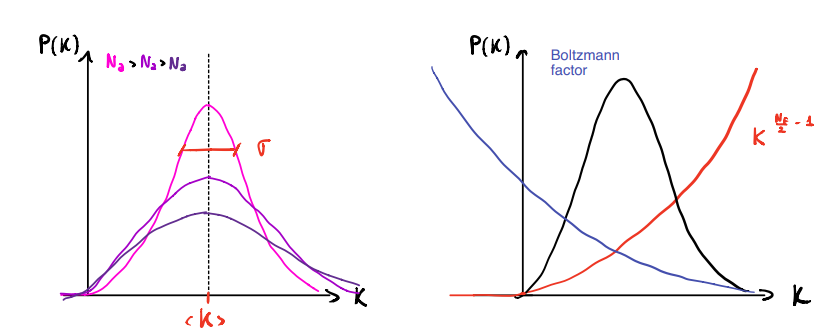
\includegraphics[width=0.7\textwidth]{Thermostats/images/kinetic distribution.PNG}
    \caption{On the left: qualitative behaviour of the Gamma distribution $P_K(K)$ at different values of $N_a$, always centered in the same value in order to compare visually the different shapes. On the right: qualitative behaviour of the two factors that compose $P_K(K)$, whose coexistence leads to the typical shape of the Gamma distribution.}
    \label{fig:kinetic distribution}
\end{figure}

\section{Algorithms}

As mentioned in the Introduction, the two main properties of the thermostats we want to implement are:
\begin{itemize}
    \item Equilibration of the system to a target value of the temperature $\bar T$, that, after an early transient, have to remain constant;
    \item Production of configurations drawn from the Canonical ensemble.
\end{itemize}

First of all, we have seen, as one of the main results of the theoretical description of the Canonical ensemble, that \begin{math} <K> \propto T \end{math}. 
Therefore, we can think about controlling the value of the temperature through the control of the kinetic energy $K(p)$, which will have to reach the target value $\bar K \propto \bar T$. This control on $K(p)$ can be realized imposing proper variations of $K(p)$ itself, in such a way that $<K>= \bar K$. 

But this will not be sufficient in order to satisfy the second request: in fact, in order for our simulation to produce canonical configurations, we need also the fluctuations on $K(p)$ to be coherent with the canonical distribution, and so equal to its variance $\sigma_K^2$.

As a consequence of these requirements, the main idea to implement thermostats is by choosing a rule for the variation of $K(p)$, and evolving the system through a modified version of Hamilton equations, which will determine variations of potential energy $U(q)$ in such a way that the ones of $K(p)$ are balanced, and so that the total energy is approximately conserved.


\subsection{Trial and error}

The first attempt, which can not be called an actual algorithm, but is useful to introduce us to the logic underlying thermostats, is the "Trial and error". 
It exploits the behaviour of the simulation to set the proper value of the initialization $K_0$ which, after a transient, will lead to the target value \begin{math} \bar K \end{math} (and so to the target value \begin{math} \bar T \end{math}).

At first, in fact, we could try initializating the kinetic energy at its target value. Unfortunately, starting the simulation we would see that $K$ doesn't remain constant at $\bar K$, but equilibrates to a different value.

So, we could think of starting a new simulation from a different $K_0$, shifted from the previous by the difference between $\bar K$ and the previous equilibration value.
Typically, the optimal result can not be reached in a unique attempt, but after various iterations, which can be stopped when the difference between $\bar K$ and the new equilibration value of $K$ is small enough.

\begin{figure}
    \centering
    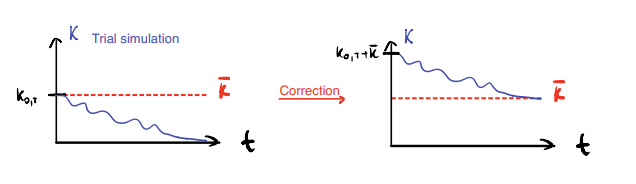
\includegraphics[width=0.7\textwidth]{Thermostats/images/Trial and error.PNG}
    \caption{The first image represent the Trial simulation, where the kinetic energy is initialized to its target value. The second represent the correct simulation, where the initialization is set to that value from which, after the equilibration, the kinetic energy reaches the target value.}
    \label{fig:trial and error}
\end{figure}

In Figure \ref{fig:trial and error} we see how this procedure would look if a unique attempt would be sufficient.

Unfortunately, as we can imagine looking at the triviality of this algorithm, this is not a suitable choice for implementing a thermostat.

\subsection{Velocity rescaling}
The Velocity rescaling algorithm is based on the following idea:
\begin{itemize}
    \item Given an initial configuration of the system, we run a number \textit {stride} of steps using a Hamilton equations integrator, like, for example, Velocity Verlet;
    \item We check the istantaneous value of $K$ and we change it rescaling it by a factor that makes it equal to the target value $\bar K=\frac{3}{2}N_a K_B \bar T$.
\end{itemize}

A pseudocode representing these operations would be:
\begin{algorithm}[H]\label{velocity_rescaling}
			\caption{Velocity rescaling algorithm}
			\begin{algorithmic}[1]
				\For{$i step\; inrange (nsteps)$}
    				\State $p+=f*\Delta t/2$
    				\State $q+=p*\Delta t/m$
    				\State $p+=f*\Delta t/2$
    				\If{$i step\%stride==0$}
    				    \State $K= \frac{\sum_{i}{p_i^2}}{{2m_i}}$
    				    \State $p* = \sqrt{\frac{\Bar{K}}{K}}$
    				\EndIf
				\EndFor
			\end{algorithmic}
		\end{algorithm}

\begin{figure}
    \centering
    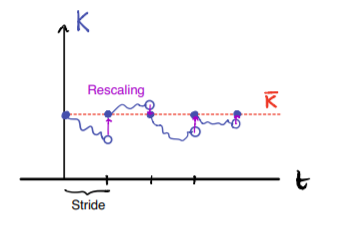
\includegraphics[width=0.7\textwidth]{Thermostats/images/velocity rescaling.PNG}
    \caption{Example of a trajectory $K(t)$ produced using the Velocity rescaling thermostat.}
    \label{fig:velocity rescaling}
\end{figure}		

As we can see, in this case the change in the kinetic energy is made on its total value, and not on the specific values $K_i$ of the single particles: this feature defines the so called \textit {Global thermostats}.

Although, as also qualitatively represented in Figure \ref{fig:velocity rescaling}, this algorithm works well in the equilibration to the target value $\bar K$, reached in a time interval $\propto {\textit {stride}}$, this is not an optimal choice for two main reasons: first of all, the distribution we are sampling from is unknown, and certainly it is not the canonical since the fluctuations of $K$ are not the proper ones (see Figure \ref{fig:fluctuations}); then, the trajectory is discontinuous, and this does not allow us to convert the algorithm into a differential equation.

\begin{figure}
    \centering
    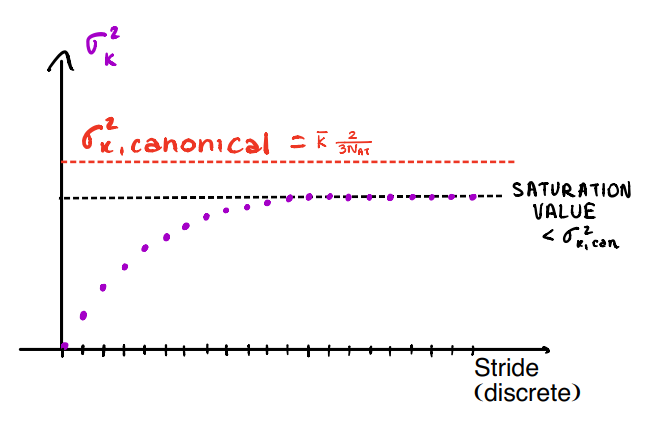
\includegraphics[width=0.7\textwidth]{Thermostats/images/fluctuations.PNG}
    \caption{Behaviour of $\sigma_K^2$ as a function of \textit {stride}. If \textit {stride} is small, the trajectory is smoother and $<K>=\bar K$, but the fluctuations are too small. If \textit{stride} is too big, the fluctuations will reach a saturation value smaller than the correct one, and also $K$ doesn't reach the target: in fact, this choice would basically correspond to evolving the system according to Velocity Verlet, which guarantees the conservation of the total energy and then produces configurations drawn from the Microcanonical distribution. }
    \label{fig:fluctuations}
\end{figure}

\subsection{Berendsen thermostat}
The problem of discontinuity in Velocity rescaling algorithm is soon solved by the Berendsen thermostat, which can be interpreted as its "continuous version".

It is based on the idea of modifying $K$ at each step, rescaling it by a properly weighted sum of the current value and the target value.

In practice, this operation would consist into the multiplication of the current value of the momentum $p$ by a factor
\begin{equation}
    F={\sqrt{\frac{c_1K+c_2 \bar K}{K}}}.
\end{equation}

In particular, the choice of the weights ${c_1}$ and ${c_2}$ has to guarantee the following properties:
\begin{itemize}
    \item $c_1+c_2=1$
    since, when $K=\bar K$, the factor F must be equal to 1, because the target value has been reached, and then we do not have to modify the current value;
    \item the limit $c_1 \rightarrow 1$ ( $\implies c_2 \rightarrow 0$), which represents the absence of the thermostat (since there are no corrections to the current values $p$) should coincide with the limit case of $\textit{stride}=\tau \rightarrow \infty$ in Velocity rescaling;
    \item the limit $c_2 \rightarrow 1$ ($\implies c_1 \rightarrow 0$), which basically respresents the application of Velocity rescaling at each step, should coincide with the limit case of $\textit{stride}=\tau \rightarrow 0$.
\end{itemize}

A choice which guarantees the latter requests is:
\begin{equation}
   c_1=e^{-{\frac{\Delta t}{\tau}}} ;\quad
      c_2=1-c_1=1-e^{-{\frac{\Delta t}{\tau}}}
\end{equation}

At this point, we can try converting the algorithm into a differential equation:
\begin{multline*}
    K_{new}={\frac{e^{-{\frac{\Delta t}{\tau}}}K+\left(1-e^{-{\frac{\Delta t}{\tau}}}\right) \bar K}{K}}K \\ 
    \implies \Delta K=K_{new}-K=e^{-{\frac{\Delta t}{\tau}}}K + (1-e^{-{\frac{\Delta t}{\tau}}}) \bar K - K \\
    = (1-e^{-{\frac{\Delta t}{\tau}}} )(\bar K -K) 
\end{multline*}

Then, performing the infinitesimal limit:
\begin{equation*}
    \lim_{{\Delta t}\to 0} \Delta K = (1-1+\frac{\Delta t}{\tau} + \textit{h.o.t})(\bar K-K)=\frac{\Delta t}{\tau}(\bar K-K)
\end{equation*}

\begin{equation}
    \implies dK=dt \frac{(\bar K-K)}{\tau}
\end{equation}

that is actually a differential equation. This means its solution, i.e. $K(t)$, is continuous, and then we can say that the issue we had with Velocity rescaling is solved.

Another advantage with respect to Velocity rescaling is that now we have a control parameter $\tau$, which, differently from \textit{stride}, has a physical interpretation:
it is the relaxation time of the system, and gives a qualitative measure of the thermal inertia of it, since the greater is $\tau$, the more difficult will be to change $K$, namely $T$.

Moreover, as a smoother version of Velocity rescaling, Berendsen's is itself a global thermostat.

So, in conclusion, one of the main advantages of using this algorithm is that the trajectories it produces are continuous, but it is not the only one. In fact, according to the huge number of citations of the original paper by Berendsen (1984), it is probably the most used thermostat, and this is due to a series of properties: it empirically equilibrates well; it is easy to understand; it is efficient. Regarding the efficiency, this is what actually makes people prefer this algorithm to more exact ones like, for example, Hybrid Montecarlo: indeed, the approximation makes Berendsen thermostat quicker in simulating very large systems, for  which a more accurate algorithm would take a too long time.

However, this algorithm does not sample configurations from the canonical distribution. In fact, even if balance is satisfied, because a stationary distribution can be reached, this is not the canonical one, and this is due to the fact that $K$ does not respect the proper fluctuations. Detailed balance is instead not guaranteed, because $K$ is forced to reach $\bar K$ and a time-reversed trajectory is not even possible.



